\subsection{MLCommons Medical AI - Brain Tumor Segmentation (BraTS)}
{{\footnotesize
\noindent The MLCommons Medical AI working group develops benchmarks, best practices, and platforms (MedPerf, GaNDLF, COFE)
to accelerate robust, privacy-preserving AI development for healthcare. MedPerf enables federated testing of clinical
models on diverse datasets, improving generalizability and equity while keeping data onsite .


\begin{description}[labelwidth=4cm, labelsep=1em, leftmargin=4cm, itemsep=0.1em, parsep=0em]
  \item[date:] 2023-07-17
  \item[version:] v1.0
  \item[last\_updated:] 2023-07
  \item[expired:] unknown
  \item[valid:] yes
  \item[valid\_date:] 2023-07-17
  \item[url:] \href{https://github.com/mlcommons/medical}{https://github.com/mlcommons/medical}
  \item[doi:] 10.1038/s42256-023-00652-2
  \item[domain:]
    - Biology \& Medicine
  \item[focus:] Federated benchmarking and evaluation of medical AI models across diverse real-world clinical data
  \item[keywords:]
    - medical AI
    - federated evaluation
    - privacy-preserving
    - fairness
    - healthcare benchmarks
  \item[licensing:] Apache License 2.0
  \item[task\_types:]
    - Federated evaluation
    - Model validation
  \item[ai\_capability\_measured:]
    - Clinical accuracy
    - fairness
    - generalizability
    - privacy compliance
  \item[metrics:]
    - ROC AUC
    - Accuracy
    - Fairness metrics
  \item[models:]
    - MedPerf-validated CNNs
    - GaNDLF workflows
  \item[ml\_motif:]
    - Classification
  \item[type:] Platform
  \item[ml\_task:]
    - NA
  \item[solutions:] 0
  \item[notes:] Open-source platform under Apache-2.0; used across 20+ institutions and hospitals .

  \item[contact.name:] Alex Karargyris (MLCommons Medical AI)
  \item[contact.email:] unknown
  \item[datasets.links.name:] Multi-institutional clinical datasets, radiology
  \item[results.links.name:] ChatGPT LLM
  \item[fair.reproducible:] Yes
  \item[fair.benchmark\_ready:] Yes
  \item[id:] mlcommons\_medical\_ai\_-\_brain\_tumor\_segmentation\_brats
  \item[Citations:] \cite{karargyris2023federated}
\end{description}

{\bf Ratings:} ~ \\

\begin{tabular}{p{0.15\textwidth} p{0.07\textwidth} p{0.7\textwidth}}
\hline
Rating & Value & Reason \\
\hline
dataset & 4 & Multi-institutional datasets used in federated settings; real-world data is handled
privately onsite, but some FAIR aspects (e.g., accessibility and metadata) are implicit.
 \\
documentation & 5 & Extensive documentation, papers, and community support exist. Clear examples and usage
instructions are provided in GitHub and publications.
 \\
metrics & 5 & Metrics such as ROC AUC, accuracy, and fairness are clearly specified and directly
support goals like generalizability and equity.
 \\
reference\_solution & 3 & GaNDLF workflows and MedPerf-validated CNNs are referenced, but not all baseline models
are centrally documented or easily reproducible.
 \\
software & 5 & GitHub repository (https://github.com/mlcommons/medical) provides actively maintained
open-source tools like MedPerf and GaNDLF for federated medical AI evaluation.
 \\
specification & 4 & The platform defines federated tasks and model evaluation scenarios. Some clinical and
system-level constraints are implied but not uniformly formalized across all use cases.
 \\
\hline
\end{tabular}

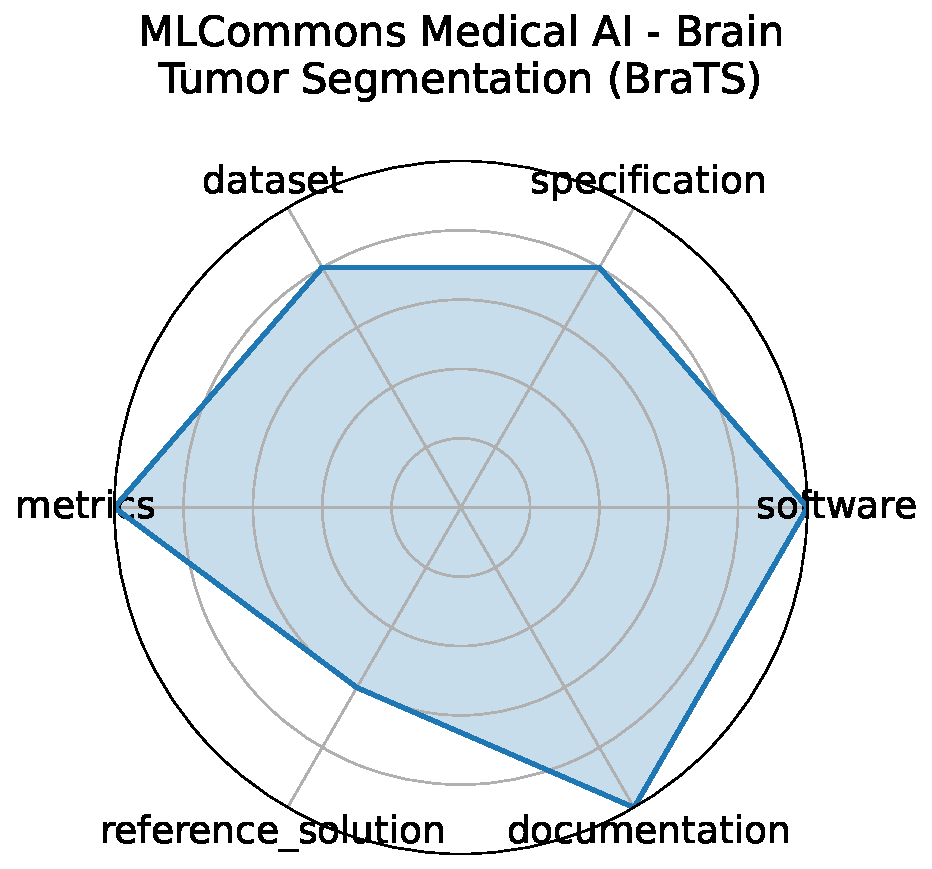
\includegraphics[width=0.2\textwidth]{mlcommons_medical_ai_-_brain_tumor_segmentation_brats_radar.pdf}
}}
\clearpage